\chapter{Core periphery structure} 

Rombach Core periphery revisited – generates continues value coreness for each node

Borgatti and Everett

Hubs are commonly found in empirical networks and pose a problem for community detection as they usually have strong ties to many communities. Identifying core–periphery structures can help circumvent this problem by categorizing hubs as part of the network's core (Rombach et al., 2014, p. 160).  (from Wikipedia)

ref Rombach, M. P., Porter, M. A., Fowler, J. H., \& Mucha, P. J. (2014). Core–periphery structure in Networks. SIAM J. Appl. Math., 74(1), 167–190.

Chung and Lu power law random graph with beta element [2,3] contains core

from Rombach
Core (hub) nodes can have strong ties to different communities

Communities as tiles that overlap to produce network core Yang and Leskovec

Original paper

1 Intuitively different concepts can bemathematically similar eg global core periphery with local community structure, globaql community structure with local core peripehry and network with multiple core periphery pairs

II search for various cores with a sizer and shape parameter (rather than a global optimum like odularity)

Core periphery strcutre is often correlated with measures sucha s degree centrality, eigenvector centrality, betweenness centrality and page rank although these are intuitively different concepts

also different from rich clubs (see Zhang and Newman)

Borgatti and Everett have a multi core model too (in bib ccohesive subsets)

Kojaku and Masuda also have algorithm for multiple cores (GR and cdode for a significance test for networks)

Zhang and Newman use block model which has also been used by Peixoto to study core periphery (including nested)

Spectral partitioning for core periphery
Cucuringu adjacency as low rank perturbation matrix
Barucca spectral regularities for core periphery

Some spectral methods rely on edge density (bit like community structure)
others transport where core nodes are likeloy to be on shortest paths
Curucuringu again and Lee, Cucuringu and Porter use a transport based coreness

k core fast but like requiring a community to be a network clique



Other cp

Luo 2009 Core periphery in PPI

Other stuff

Benchmarks


TTD
Coreness in igraph seems to pick ou (surprisingly core nodes – lethality etc inc housekeeping) and peripheral (more specifically synaptic associated with transmission).
Add to centrality measures
Try enrichment gmt with removal of k core
Try induced subgraph with k core removed



\section{Introduction}
\subsection{The leading eigenvector and coreness}
The principle eigenvector is all negative in the graph it is also all negative in core periphery structures
There is a linera relationship with both betweeness centrality but more particularly degree

So I have read about this today and it is a consequence of Perron-Frobenius theorem
If you select the most negative values you pick out a lot of ribosomal components and get very strong enrichment for GO categories.
Disease ontologies are neoplastic and these genes are essential

Low values gets epilepsies, lots of specific neuronal transmitter stuff

\todo{do with background PSP}
If you take the row eig eig\$vector[1, ] you get the sign of all the eigenvectors for that gene. It is symmetrical too about the midline (?because matrix symmetrical and of equal values)

Lowest quartile of second eigenvector - lots of actin and cytoskeletal, schizo and adhd

highest quartile of second eigenvector - RNA binding, ribosome, lethality, non homogenous diseases


Lowest 230 ish of second eigenvetor - 80 actin binding and 54 cadherin

5th lowest centile 2nd eigenvector - 72 actin binding 45 cadherin

Pseudo spokes have low principle eigenvectors

Pseudo hubs have lower leading eigenvector than overall but less than pseudospokes

Ps vs ph
W = 1602, p-value = 0.03092
Wilcoxon

wilcox.test(eig\_filter\_ph,vec)

        Wilcoxon rank sum test with continuity correction

data:  eig\_filter\_ph and vec
W = 19194, p-value = 5.552e-06
alternative hypothesis: true location shift is not equal to 0

> wilcox.test(eig\_filter,vec)

        Wilcoxon rank sum test with continuity correction

data:  eig\_filter and vec
W = 42907, p-value < 2.2e-16
alternative hypothesis: true location shift is not equal to 0
\section{SNAP}

\subsection{Previous}
The file \url{/home/grant/Dropbox/PhD/Core\_Periphery/SBM\_snap.odt}

Shows that the maximum likelihood is at 5 groups in SNAP. I have not yet located the gml. From memory these are overlapping. I think this might have been a graph from making a five group planted SBM.

The snap single core single periphery gmt file is at MAC \url{ gene\_set/ctg\_PSP\_3457\_SNAP\_core\_and\_complement.gmt.sets.out}

There is a sbm\_2\_group in utils R on laptop which I think is when I made a sbm with two groups to find if it had a core periphery structure.

\url{~/RProjects/utils/src/generic_compile_gsa_original_SNAP.R} gets you the ed and int for the core periphery.

\subsection{Redo}

\url{source('~/RProjects/core_snapR/R/2_get_inner_core.R')}
Code to run snap
\url{/home/grant/Programs/snap/examples/bigclam/phd_bigclam.sh} or \url{phd_coregraph_bigclam.sh}

I have done for core, inner core and periphery

Periphery very much receptors associated with neurological disease, outer core more neurodegenerative, inner core nasy and early

Structure is very similar to kcore with high k in inner core. Makes complete subgraph therefore backs up what Yang and Leskovec say about core periphery. 

% latex table generated in R 3.6.1 by xtable 1.8-4 package
% Sat Jan  4 15:50:54 2020
\begin{table}[ht]
\centering
\begin{tabular}{rlrrrrrr}
  \hline
 & SET & NGENES & BETA & BETA\_STD & SE & P & P\_C \\ 
  \hline
1 & outer\_snap3457\_Jan10005 &  1276 & 0.1080 & 0.0274 & 0.0287 & 0.0001 & 0.0700 \\ 
  2 & middle1000 &  1717 & 0.0530 & 0.0155 & 0.0244 & 0.0149 & 0.0045 \\ 
  3 & inner10006 &   305 & 0.0040 & 0.0005 & 0.0531 & 0.4697 & 0.2298 \\ 
   \hline
\end{tabular}
\caption{MAGMA enrichment for Intelligence by SNAP core layer} 
\label{Table:MAGMA enrichment for Intelligence by SNAP core layer}
\end{table}

% latex table generated in R 3.6.1 by xtable 1.8-4 package
% Sat Jan  4 15:55:54 2020
\begin{table}[ht]
\centering
\begin{tabular}{rlrrrrrr}
  \hline
 & SET & NGENES & BETA & BETA\_STD & SE & P & P\_EA2 \\ 
  \hline
1 & outer\_snap3457\_Jan10005 &  1276 & 0.0283 & 0.0072 & 0.0294 & 0.1681 & 0.1041 \\ 
  2 & middle1000 &  1717 & 0.0807 & 0.0235 & 0.0250 & 0.0006 & 0.0569 \\ 
  3 & inner10006 &   305 & -0.0277 & -0.0036 & 0.0544 & 0.6946 & 0.0276 \\ 
   \hline
\end{tabular}
\caption{MAGMA enrichment for Education by SNAP core layer} 
\label{Table:MAGMA enrichment for Education by SNAP core layer}
\end{table}
% latex table generated in R 3.6.1 by xtable 1.8-4 package
% Sat Jan  4 15:55:54 2020
\begin{table}[ht]
\centering
\begin{tabular}{rlrrrrr}
  \hline
 & SET & NGENES & BETA & BETA\_STD & SE & P \\ 
  \hline
1 & outer\_snap3457\_Jan10005 &  1274 & 0.0739 & 0.0189 & 0.0368 & 0.0222 \\ 
  2 & middle1000 &  1716 & 0.0976 & 0.0286 & 0.0310 & 0.0008 \\ 
  3 & inner10006 &   305 & 0.1880 & 0.0242 & 0.0680 & 0.0028 \\ 
   \hline
\end{tabular}
\caption{MAGMA enrichment for EA3 by SNAP core layer} 
\label{Table:MAGMA enrichment for EA3 by SNAP core layer}
\end{table}
% latex table generated in R 3.6.1 by xtable 1.8-4 package
% Sat Jan  4 15:55:54 2020
\begin{table}[ht]
\centering
\begin{tabular}{rlrrrrr}
  \hline
 & SET & NGENES & BETA & BETA\_STD & SE & P \\ 
  \hline
1 & outer\_snap3457\_Jan10005 &  1329 & 0.1250 & 0.0320 & 0.0305 & 0.0000 \\ 
  2 & middle1000 &  1765 & 0.0908 & 0.0266 & 0.0259 & 0.0002 \\ 
  3 & inner10006 &   317 & 0.0300 & 0.0039 & 0.0567 & 0.2984 \\ 
   \hline
\end{tabular}
\caption{MAGMA enrichment for EA3 by SNAP core layer} 
\label{Table:MAGMA enrichment for EA3 by SNAP core layer}
\end{table}
% latex table generated in R 3.6.1 by xtable 1.8-4 package
% Sat Jan  4 15:55:54 2020
\begin{table}[ht]
\centering
\begin{tabular}{rlrrrrr}
  \hline
 & SET & NGENES & BETA & BETA\_STD & SE & P \\ 
  \hline
1 & outer\_snap3457\_Jan10005 &  1329 & 0.1250 & 0.0320 & 0.0305 & 0.0000 \\ 
  2 & middle1000 &  1765 & 0.0908 & 0.0266 & 0.0259 & 0.0002 \\ 
  3 & inner10006 &   317 & 0.0300 & 0.0039 & 0.0567 & 0.2984 \\ 
   \hline
\end{tabular}
\caption{MAGMA enrichment for EA3 by SNAP core layer} 
\label{Table:MAGMA enrichment for EA3 by SNAP core layer}
\end{table}
\todo{get core periphery probabilities for snap and different kcore}

\todo{PLI for cores}

\todo{Do gephi of core, periphery inner core}
\section{Stochastic block model}

\url{~/RProjects/utils/src/sbm_first_level_resultsfunc.R}
\url{/Users/grantrobertson/PycharmProjects/newmam_core_periphery/newman_core/sbm_nested.py}

One can fit a nested block stochastic model. Maximising the log likelihood of the model is equivalent to minimising the entropy of the ensembl \cite{peixoto2014hierarchical}.

The blocks of the nested sbm were 54 in numbrt for the first level, 7 for the clustering of the 54 blocks and all were combined in level 2. 

Enrichment results using MAGMA for intelligence discovery and replication cohorts are shown in table \ref{table:SBM_intelligence}. 

The results for enrichment using MAGMA for education discovery and replication cohorts are shown in table \ref{table:SBM_level0_ed}

6 gene sets achieved nominal significance in the discovery cohort for intelligence and education. Group 17 is significant in the intelligence replication cohort but not in the education replication. However using the EA3 cohort it is significant with p=0.005.

code for tables \url{source('~/RProjects/utils/src/generic_compile_sbm_level0_redo.R'}

The modularity of the partition is 0.11. Random permutation of community lables resulted in a modularity of approx 0 \todo{more replications}

\todo{Is the modularity low because the sets overlap?. What is the modularity of the higher level partiion? The sets seem to have a narrower range of sizes at the bottom level}
Gene ontology enrichment analysis with topgene shows significant enrichment for glutamate receptor activity GO:0008066	glutamate receptor activity		Bonferroni	1.064E-39	28 found	84 in annotation.  number of genes in set 117 code for gene set to clipboard \url{source('~/RProjects/utils/src/go_enrichment_sbm/calculate_modularity_sbm.R')}

\todo{GO with background of PSP and overlap group 5 and 17}

% latex table generated in R 3.6.1 by xtable 1.8-4 package
% Wed Jan  1 17:16:22 2020
\begin{table}[ht]
\centering
\begin{tabular}{lrrrrrr}
  \hline
SET & NGENES & BETA & BETA\_STD & SE & P DISCOVERY & P REPLICATION \\ 
  \hline
0: &   31 & -0.095 & -0.004 & 0.177 & 0.704 & 0.706 \\ 
  1: &  880 & 0.072 & 0.015 & 0.034 & 0.018 & 0.146 \\ 
  2: &   61 & -0.046 & -0.003 & 0.128 & 0.640 & 0.072 \\ 
  4: &   54 & 0.144 & 0.008 & 0.141 & 0.155 & 0.164 \\ 
  5: &  105 & 0.026 & 0.002 & 0.089 & 0.387 & 0.706 \\ 
  6: &  180 & 0.071 & 0.007 & 0.070 & 0.158 & 0.369 \\ 
  7: &  101 & 0.094 & 0.007 & 0.092 & 0.153 & 0.129 \\ 
  8: &   85 & -0.063 & -0.004 & 0.103 & 0.731 & 0.147 \\ 
  9: &   36 & 0.097 & 0.004 & 0.152 & 0.261 & 0.487 \\ 
  10: &  127 & 0.229 & 0.019 & 0.088 & 0.005 & 0.112 \\ 
  11: &   41 & 0.025 & 0.001 & 0.137 & 0.429 & 0.912 \\ 
  12: &   55 & -0.007 & -0.000 & 0.134 & 0.520 & 0.877 \\ 
  14: &   66 & 0.014 & 0.001 & 0.112 & 0.450 & 0.512 \\ 
  15: &  132 & -0.066 & -0.006 & 0.086 & 0.778 & 0.782 \\ 
  16: &   26 & 0.020 & 0.001 & 0.188 & 0.458 & 0.029 \\ 
  17: &  109 & 0.311 & 0.024 & 0.102 & \textbf{0.001} & \textbf{0.010} \\ 
  18: &  103 & 0.132 & 0.010 & 0.090 & 0.073 & 0.187 \\ 
  19: &   39 & -0.233 & -0.011 & 0.166 & 0.920 & 0.306 \\ 
  20: &   30 & 0.163 & 0.007 & 0.167 & 0.165 & 0.433 \\ 
  21: &   54 & 0.286 & 0.015 & 0.118 & 0.008 & 0.090 \\ 
  22: &   18 & 0.076 & 0.002 & 0.203 & 0.354 & 0.809 \\ 
  23: &   74 & 0.188 & 0.012 & 0.104 & 0.036 & 0.771 \\ 
  24: &   33 & 0.121 & 0.005 & 0.135 & 0.185 & 0.780 \\ 
  25: &   48 & 0.074 & 0.004 & 0.139 & 0.297 & 0.089 \\ 
  26: &   84 & 0.078 & 0.005 & 0.101 & 0.222 & 0.182 \\ 
  27: &   19 & 0.316 & 0.010 & 0.222 & 0.077 & 0.048 \\ 
  28: &   50 & -0.197 & -0.010 & 0.150 & 0.905 & 0.058 \\ 
  29: &   62 & 0.014 & 0.001 & 0.117 & 0.453 & 0.047 \\ 
  30: &   24 & 0.346 & 0.013 & 0.183 & 0.029 & 0.466 \\ 
  31: &   55 & 0.079 & 0.004 & 0.135 & 0.280 & 0.705 \\ 
  35: &   76 & 0.026 & 0.002 & 0.113 & 0.408 & 0.697 \\ 
  37: &   40 & 0.015 & 0.001 & 0.149 & 0.461 & 0.011 \\ 
  39: &   50 & 0.135 & 0.007 & 0.131 & 0.151 & 0.860 \\ 
  40: &   18 & 0.035 & 0.001 & 0.242 & 0.443 & 0.493 \\ 
  41: &   40 & -0.005 & -0.000 & 0.142 & 0.514 & 0.737 \\ 
  43: &   18 & 0.018 & 0.001 & 0.220 & 0.467 & 0.687 \\ 
  45: &   28 & -0.135 & -0.005 & 0.172 & 0.783 & 0.099 \\ 
  47: &   24 & 0.151 & 0.005 & 0.197 & 0.222 & 0.612 \\ 
  50: &   21 & -0.480 & -0.016 & 0.210 & 0.989 & 0.134 \\ 
  51: &   44 & 0.011 & 0.001 & 0.153 & 0.471 & 0.062 \\ 
  52: &   20 & -0.103 & -0.003 & 0.216 & 0.684 & 0.465 \\ 
   \hline
\end{tabular}
\caption{MAGMA GSA level 0 Stochastic block model. Intelligence} 
\label{table:SBM_intelligence}
\end{table}

% latex table generated in R 3.6.1 by xtable 1.8-4 package
% Wed Jan  1 17:26:36 2020
\begin{table}[ht]
\centering
\begin{tabular}{lrrrrrr}
  \hline
SET & NGENES & BETA & BETA\_STD & SE & P & P\_EA2 \\ 
  \hline
0: &   31 & 0.253 & 0.010 & 0.181 & 0.081 & 0.028 \\ 
  1: &  880 & 0.075 & 0.016 & 0.035 & 0.017 & 0.439 \\ 
  2: &   61 & -0.127 & -0.007 & 0.131 & 0.834 & 0.535 \\ 
  4: &   54 & 0.192 & 0.010 & 0.145 & 0.092 & 0.144 \\ 
  5: &  105 & -0.032 & -0.002 & 0.092 & 0.637 & 0.579 \\ 
  6: &  180 & -0.073 & -0.007 & 0.072 & 0.844 & 0.779 \\ 
  7: &  101 & 0.140 & 0.010 & 0.094 & 0.067 & 0.386 \\ 
  8: &   85 & -0.133 & -0.009 & 0.105 & 0.898 & 0.461 \\ 
  9: &   36 & -0.021 & -0.001 & 0.155 & 0.555 & 0.119 \\ 
  10: &  127 & 0.080 & 0.007 & 0.090 & 0.188 & 0.203 \\ 
  11: &   41 & 0.041 & 0.002 & 0.140 & 0.386 & 0.428 \\ 
  12: &   55 & 0.036 & 0.002 & 0.137 & 0.396 & 0.609 \\ 
  14: &   66 & -0.072 & -0.004 & 0.115 & 0.733 & 0.053 \\ 
  15: &  132 & -0.028 & -0.002 & 0.088 & 0.624 & 0.262 \\ 
  16: &   26 & 0.487 & 0.018 & 0.193 & 0.006 & 0.176 \\ 
  17: &  109 & 0.255 & 0.020 & 0.105 & \textbf{0.007} & 0.447 \\ 
  18: &  103 & -0.166 & -0.012 & 0.093 & 0.963 & 0.156 \\ 
  19: &   39 & 0.005 & 0.000 & 0.170 & 0.489 & 0.532 \\ 
  20: &   30 & 0.181 & 0.007 & 0.171 & 0.145 & 0.473 \\ 
  21: &   54 & -0.045 & -0.002 & 0.120 & 0.646 & 0.443 \\ 
  22: &   18 & 0.183 & 0.006 & 0.208 & 0.190 & 0.831 \\ 
  23: &   74 & 0.061 & 0.004 & 0.107 & 0.282 & 0.154 \\ 
  24: &   33 & -0.059 & -0.003 & 0.139 & 0.666 & 0.090 \\ 
  25: &   48 & 0.038 & 0.002 & 0.142 & 0.394 & 0.391 \\ 
  26: &   84 & 0.116 & 0.008 & 0.104 & 0.132 & 0.084 \\ 
  27: &   19 & 0.200 & 0.006 & 0.227 & 0.189 & 0.335 \\ 
  28: &   50 & 0.051 & 0.003 & 0.154 & 0.371 & 0.379 \\ 
  29: &   62 & 0.280 & 0.016 & 0.120 & 0.010 & 0.368 \\ 
  30: &   24 & 0.188 & 0.007 & 0.187 & 0.157 & 0.697 \\ 
  31: &   55 & -0.122 & -0.007 & 0.138 & 0.811 & 0.503 \\ 
  35: &   76 & 0.125 & 0.008 & 0.116 & 0.139 & 0.929 \\ 
  37: &   40 & 0.286 & 0.013 & 0.152 & 0.030 & 0.757 \\ 
  39: &   50 & -0.034 & -0.002 & 0.134 & 0.600 & 0.648 \\ 
  40: &   18 & 0.495 & 0.015 & 0.248 & 0.023 & 0.719 \\ 
  41: &   40 & -0.193 & -0.009 & 0.146 & 0.907 & 0.184 \\ 
  43: &   18 & 0.081 & 0.003 & 0.225 & 0.359 & 0.584 \\ 
  45: &   28 & 0.114 & 0.004 & 0.176 & 0.260 & 0.499 \\ 
  47: &   24 & 0.126 & 0.005 & 0.202 & 0.267 & 0.284 \\ 
  50: &   21 & 0.307 & 0.010 & 0.215 & 0.077 & 0.144 \\ 
  51: &   44 & -0.100 & -0.005 & 0.156 & 0.740 & 0.002 \\ 
  52: &   20 & -0.152 & -0.005 & 0.221 & 0.754 & 0.070 \\ 
   \hline
\end{tabular}
\caption{MAGMA GSA level 00 Stochastic block model for Education } 
\label{Table:SBM_education}
\end{table}

% latex table generated in R 3.6.1 by xtable 1.8-4 package
% Wed Jan  1 17:37:50 2020
\begin{table}[ht]
\centering
\begin{tabular}{lrrrrr}
  \hline
SET & NGENES & BETA & BETA\_STD & SE & P \\ 
  \hline
0: &   31 & 0.468 & 0.019 & 0.230 & 0.021 \\ 
  1: &  879 & 0.082 & 0.018 & 0.044 & 0.031 \\ 
  2: &   60 & 0.380 & 0.022 & 0.158 & 0.008 \\ 
  4: &   54 & 0.049 & 0.003 & 0.174 & 0.388 \\ 
  5: &  105 & -0.100 & -0.008 & 0.118 & 0.802 \\ 
  6: &  180 & -0.085 & -0.008 & 0.088 & 0.834 \\ 
  7: &  101 & 0.147 & 0.011 & 0.120 & 0.109 \\ 
  8: &   85 & -0.163 & -0.011 & 0.132 & 0.892 \\ 
  9: &   36 & 0.021 & 0.001 & 0.194 & 0.458 \\ 
  10: &  127 & 0.183 & 0.015 & 0.111 & 0.050 \\ 
  11: &   41 & 0.004 & 0.000 & 0.172 & 0.490 \\ 
  12: &   55 & -0.076 & -0.004 & 0.173 & 0.670 \\ 
  14: &   66 & -0.060 & -0.004 & 0.144 & 0.660 \\ 
  15: &  132 & 0.140 & 0.012 & 0.109 & 0.098 \\ 
  16: &   25 & 0.328 & 0.012 & 0.225 & 0.073 \\ 
  17: &  109 & 0.338 & 0.026 & 0.131 & 0.005 \\ 
  18: &  103 & 0.078 & 0.006 & 0.114 & 0.247 \\ 
  19: &   39 & 0.083 & 0.004 & 0.205 & 0.343 \\ 
  20: &   30 & 0.022 & 0.001 & 0.219 & 0.460 \\ 
  21: &   54 & 0.168 & 0.009 & 0.143 & 0.120 \\ 
  22: &   18 & -0.208 & -0.007 & 0.262 & 0.786 \\ 
  23: &   74 & 0.077 & 0.005 & 0.131 & 0.278 \\ 
  24: &   33 & -0.105 & -0.004 & 0.196 & 0.704 \\ 
  25: &   48 & 0.173 & 0.009 & 0.175 & 0.162 \\ 
  26: &   84 & -0.071 & -0.005 & 0.130 & 0.708 \\ 
  27: &   19 & 0.510 & 0.017 & 0.272 & 0.031 \\ 
  28: &   50 & -0.015 & -0.001 & 0.191 & 0.532 \\ 
  29: &   62 & 0.263 & 0.015 & 0.154 & 0.045 \\ 
  30: &   24 & 0.634 & 0.023 & 0.249 & 0.005 \\ 
  31: &   55 & 0.036 & 0.002 & 0.172 & 0.416 \\ 
  35: &   76 & 0.069 & 0.004 & 0.149 & 0.322 \\ 
  37: &   40 & 0.032 & 0.001 & 0.204 & 0.439 \\ 
  39: &   50 & -0.200 & -0.011 & 0.168 & 0.883 \\ 
  40: &   18 & 0.115 & 0.004 & 0.263 & 0.331 \\ 
  41: &   40 & -0.052 & -0.002 & 0.180 & 0.614 \\ 
  43: &   18 & -0.029 & -0.001 & 0.277 & 0.541 \\ 
  45: &   28 & 0.408 & 0.016 & 0.234 & 0.041 \\ 
  47: &   24 & 0.001 & 0.000 & 0.253 & 0.498 \\ 
  50: &   21 & 0.070 & 0.002 & 0.263 & 0.394 \\ 
  51: &   44 & 0.557 & 0.027 & 0.199 & 0.003 \\ 
  52: &   20 & 0.225 & 0.007 & 0.264 & 0.198 \\ 
   \hline
\end{tabular}
\caption{MAGMA GSA level 00 Stochastic block model for Education EA3} 
\end{table}
The entropy of the partition is 138146.76976646399
The number of blocks were as follows
l: 0, N: 3457, B: 54
l: 1, N: 54, B: 7
l: 2, N: 7, B: 1

\section{Two group sbm}
Seems to have core periphery structure 
code \url{source('~/RProjects/utils/src/generic_compile_gsa_core_periphery.R')} MAC

code snap core periphery \url{source('~/RProjects/utils/src/generic_compile_gsa_original_SNAP.R')}

code ortholog

\url{source('~/RProjects/utils/src/generic_compile_ortholog.R')}

code dolphin graph

\url{ source('~/RProjects/graph_analysis/R/get_famous_graphs.R')}

\section{Newman}
Newman proposes a method for detecting core based on the probability of links between edges. The implementation is described in the paper but no code is made available. Code from one of the authors corresponding to this is found in \todo{url}. There are some minor issues in the python script that do not allow it to run. I have converted it to python 3 and fixed these minor errors. While the script works well with the examples given (eg Zachary karates set) it fails to complete after x hour requiring 12\% CPU time on workstation and with runtime warning on invalid value encountered in double\_scalars

Testing the code on a random core periphery graph generated in igraph using a stochastic block model the code fails to complete and gives divide by zero encountered in log errors with a 100 vertex graph (zachary karate club has 33).\footnote{I can find no other implementation of the algorithm and at the moment I do not have time to rewrite it. There seem to be two problems: first there is some sort of numerical overflow in one of the exp log arguments and secondly there are numerous nested loops (over 12 in three blocks) within the single function used to calculate belief propogation. I do not at present have time to rewrite this but I may do after completion and add as correction.}


\section{Core by betweenness}

\section{k coreness}

\section{Orthologs and core periphery}



\begin{figure}[h]
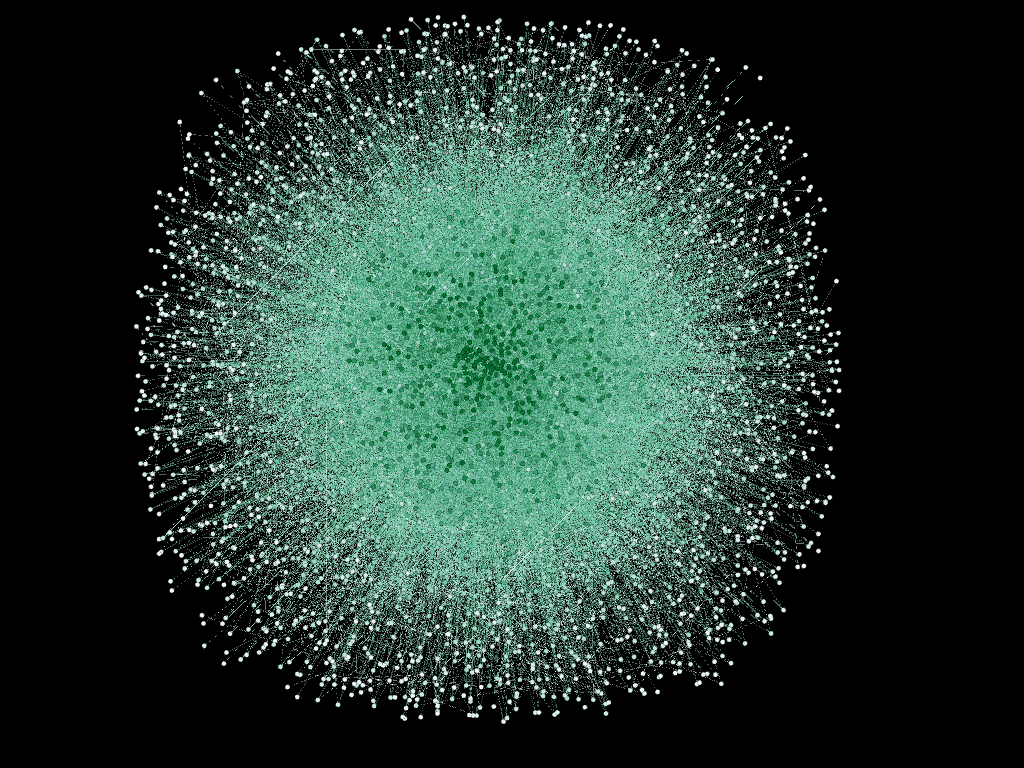
\includegraphics[width=16cm]{kcore.png}
\caption{Figure of 3457 PSP. Fruchterman Rheingold layout. Vertices coloured by coreness from dark green (high) to white (low). Coreness range 1-24. A central core is clearly seen in the physics based layout with a greater density of high kcore vertices. Gephi image in \url{~/Dropbox/stront_share/new_gephi/PSP_3457_coreness_Frucht_core_periphery.gephi
}}
\label{Fig:kcoreness}
\end{figure}

\todo{Calculate kcore correlation with p val - treat as a vertex index}


